\chapter{Benchmark against RSiena}
\label{ch:benchmark}

% generated by benchmark/make_tables.py - do not edit
\newcommand{\benchNtwoSp}{1.9}
\newcommand{\benchRfourNw}{73}
\newcommand{\benchRfourRs}{173}
\newcommand{\benchRfourSaveTwelve}{20}
\newcommand{\benchcommit}{8637ffc}
\newcommand{\benchfails}{0}
\newcommand{\benchfits}{88}
\newcommand{\benchmachine}{Apple M5 Pro (18 cores), macOS 26.5.1}
\newcommand{\benchmaxdiff}{0.07}
\newcommand{\benchmeandiff}{0.02}
\newcommand{\benchnmodels}{20}
\newcommand{\benchnparams}{152}
\newcommand{\benchrsiena}{1.6.6}
\newcommand{\benchrver}{4.6.0}
\newcommand{\benchseedsd}{0.04}
\newcommand{\benchseedsdmax}{0.11}
\newcommand{\benchserhi}{1.22}
\newcommand{\benchserlo}{0.86}
\newcommand{\benchspmax}{7.7}
\newcommand{\benchspmed}{2.2}
\newcommand{\benchspmin}{1.8}
\newcommand{\benchstata}{18 BE}
\newcommand{\coresRfive}{2.3}
\newcommand{\coresRfour}{1.6}
\newcommand{\coresRone}{1.5}
\newcommand{\coresmaxdiff}{0}
\newcommand{\coresmaxthreads}{10}
\newcommand{\coresvsrsmax}{4.6}
\newcommand{\coresvsrsmin}{3.0}

\graphicspath{{bench/}}

This chapter compares \nwsaom{} with RSiena on the same models and the same
data, for agreement of the estimates and for speed. The benchmark was run for
the Stata Journal article on \nwsaom{}; the numbers below are taken from it
(benchmark scripts: \texttt{benchmark/} in the article's repository,
\texttt{rsiena\_bench.R}, \texttt{nwsaom\_bench.do}, \texttt{make\_tables.py}).
Section~\ref{sec:benchextra} adds models for families that came later: two-mode networks, several networks (with and without a behavior, and with a non-directed network), and some of the newer effects.

\section{Design}

\nwsaom{} and RSiena \benchrsiena{} (R \benchrver) were run on \benchnmodels{}
models with each program's default algorithm settings. The data are the
50-actor Glasgow panel (RSiena's \texttt{s50}); the larger networks are 2, 4 or
10 disconnected copies of it ($n=100$, 200, 500). Network-only models use
conditional estimation (RSiena's default), except N7 (unconditional). Each
model was fitted with seeds 1--5 (1--3 for $n\ge 100$) in both programs, both on
a single thread (RSiena's default; \texttt{cores(1)} for \nwsaom{}). Times
are wall-clock seconds per fit on \benchmachine{}, never running the two
programs at the same time.

Models R1--R5 are applied-analysis specifications: R1 combines \texttt{outdegree},
\texttt{reciprocity}, \texttt{gwesp()}, transitive reciprocated triplets,
square-root indegree and outdegree popularity, \texttt{samex(smoke1)} and
\texttt{egox()}, \texttt{altx()}, \texttt{simx()} on alcohol use; R2 adds alcohol
as co-evolving behavior; R3 is undirected; R4 and R5 repeat R1 and R2 on 200
actors.

\paragraph{A caveat on \texttt{outPopSqrt}.} From RSiena 1.6.1 until 1.6.12 the default
internal parameter 0 of \texttt{outPopSqrt} (and of \texttt{outPop.c}, \texttt{outPopMore},
\texttt{inActSqrt} and related effects) made the statistic use start-of-period outdegrees without
the square root, while the ministep still used the square root, and RSiena did not converge on
these models. RSiena 1.6.13 corrected this: these effects now have internal parameter 1 by
default. The benchmark was run with RSiena \benchrsiena{}, so it sets the parameter to 1
explicitly, which is the documented definition and what \nwsaom{} implements.

\section{Agreement of the estimates}

\begin{table}[htbp]
\centering
\caption{\texttt{nwsaom} and RSiena 1.6.6 on the same models and data, both single-threaded:
largest difference in a mean estimate (in RSiena standard errors) and median seconds per fit}
\label{tab:bench}
\footnotesize
\begin{tabular}{l>{\raggedright\arraybackslash}p{0.30\textwidth}rrrrrr}
\toprule
 & Specification & $n$ & Waves & Max diff & \texttt{nwsaom} & RSiena & Speed-up \\
\midrule
\multicolumn{8}{l}{\textit{Network}} \\
N1 & \texttt{outdegree}, \texttt{reciprocity} & 50 & 2 & 0.02 & 0.31 & 1.33 & 4.3 \\
N2 & + \texttt{gwesp} & 50 & 3 & 0.07 & 1.46 & 2.78 & 1.9 \\
N4 & + \texttt{gwesp}, \texttt{samex()} & 50 & 3 & 0.03 & 1.52 & 3.42 & 2.2 \\
N5 & + \texttt{gwesp}, \texttt{indegpopularity}, \texttt{outactivity} & 50 & 3 & 0.07 & 2.63 & 5.02 & 1.9 \\
N6 & + \texttt{gwesp}, \texttt{egox()}, \texttt{altx()}, \texttt{simx()} & 50 & 3 & 0.06 & 1.96 & 4.99 & 2.5 \\
N7 & N2, unconditional estimation & 50 & 3 & 0.03 & 1.71 & 3.55 & 2.1 \\
\addlinespace
\multicolumn{8}{l}{\textit{Undirected}} \\
U1 & \texttt{outdegree}, default model (forcing) & 50 & 2 & 0.02 & 0.20 & 0.52 & 2.6 \\
U2 & \texttt{outdegree}, \texttt{symtype(joint)} & 50 & 2 & 0.06 & 0.23 & 1.75 & 7.7 \\
\addlinespace
\multicolumn{8}{l}{\textit{Co-evolution}} \\
C1 & N2 + alcohol: \texttt{linear}, \texttt{quadratic}, \texttt{avalt} & 50 & 3 & 0.07 & 2.60 & 7.38 & 2.8 \\
C2 & N2 + smoking: \texttt{linear}, \texttt{quadratic}, \texttt{avsim} & 50 & 3 & 0.06 & 2.75 & 8.74 & 3.2 \\
C3 & N1 + alcohol: \texttt{linear}, \texttt{avalt} & 50 & 2 & 0.04 & 0.63 & 2.74 & 4.4 \\
\addlinespace
\multicolumn{8}{l}{\textit{Realistic}} \\
R1 & full network model (see text) & 50 & 3 & 0.06 & 4.50 & 8.57 & 1.9 \\
R2 & R1 network part + alcohol co-evolution & 50 & 3 & 0.05 & 5.49 & 12.1 & 2.2 \\
R3 & undirected: \texttt{gwesp}, \texttt{samex()}, \texttt{simx()} & 50 & 2 & 0.03 & 0.66 & 1.21 & 1.8 \\
R4 & R1 & 200 & 3 & 0.05 & 72.9 & 173 & 2.4 \\
R5 & R2 & 200 & 3 & 0.07 & 87.6 & 177 & 2.0 \\
\addlinespace
\multicolumn{8}{l}{\textit{Larger networks}} \\
S100 & N2 & 100 & 3 & 0.04 & 5.90 & 11.2 & 1.9 \\
S200 & N2 & 200 & 3 & 0.04 & 25.6 & 55.2 & 2.2 \\
S500 & N2 & 500 & 3 & 0.03 & 200 & 375 & 1.9 \\
T200 & C1 & 200 & 3 & 0.05 & 41.8 & 109 & 2.6 \\
\bottomrule
\end{tabular}

\end{table}


Across all \benchnparams{} parameters the mean estimates over seeds differ
by at most \benchmaxdiff{} RSiena standard errors (on average \benchmeandiff{}),
which is the size of RSiena's own variation between seeds (median
\benchseedsd{} standard errors, at most \benchseedsdmax{}). Standard errors,
themselves simulation estimates, agree within 8\% for the network-only models;
in the co-evolution models the ratio of \nwsaom{} to RSiena standard errors
ranges from \benchserlo{} to \benchserhi{}. All \benchfits{} \nwsaom{} fits
converged by RSiena's criterion (overall maximum convergence ratio below 0.25).

\begin{figure}[htbp]
\centering
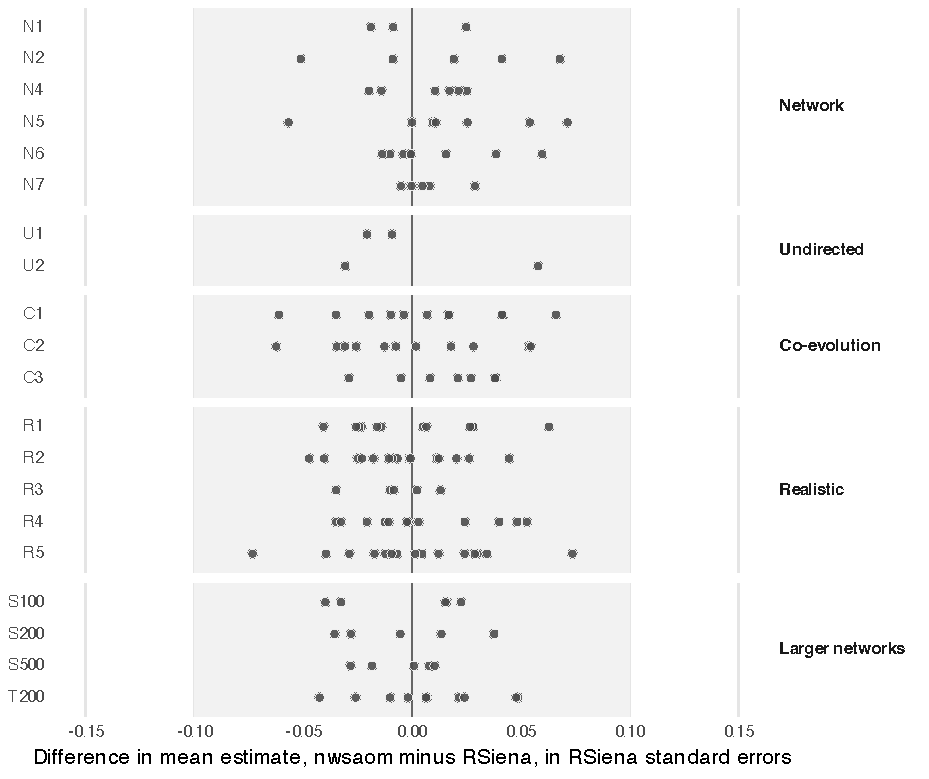
\includegraphics[width=\textwidth]{fig_bench_agree.pdf}
\caption{Difference between the mean estimates of \nwsaom{} and RSiena for every
parameter of every model, in RSiena standard errors; the band marks $\pm0.1$.}
\end{figure}

\section{Speed on one thread}

On a single thread \nwsaom{} was faster on every model, by a median factor of
\benchspmed{} (range \benchspmin--\benchspmax). The factor depends more on the
effects than on network size: models with \texttt{gwesp()} run 1.8 to 3.2 times
as fast, from 50 to 500 actors, models without it (N1, U1, U2, C3) 2.6 to 7.7
times as fast. For R4 (200 actors) one fit takes \benchRfourNw{} s against
\benchRfourRs{} s in RSiena, about \benchRfourSaveTwelve{} minutes saved over
twelve fits.

\begin{figure}[htbp]
\centering
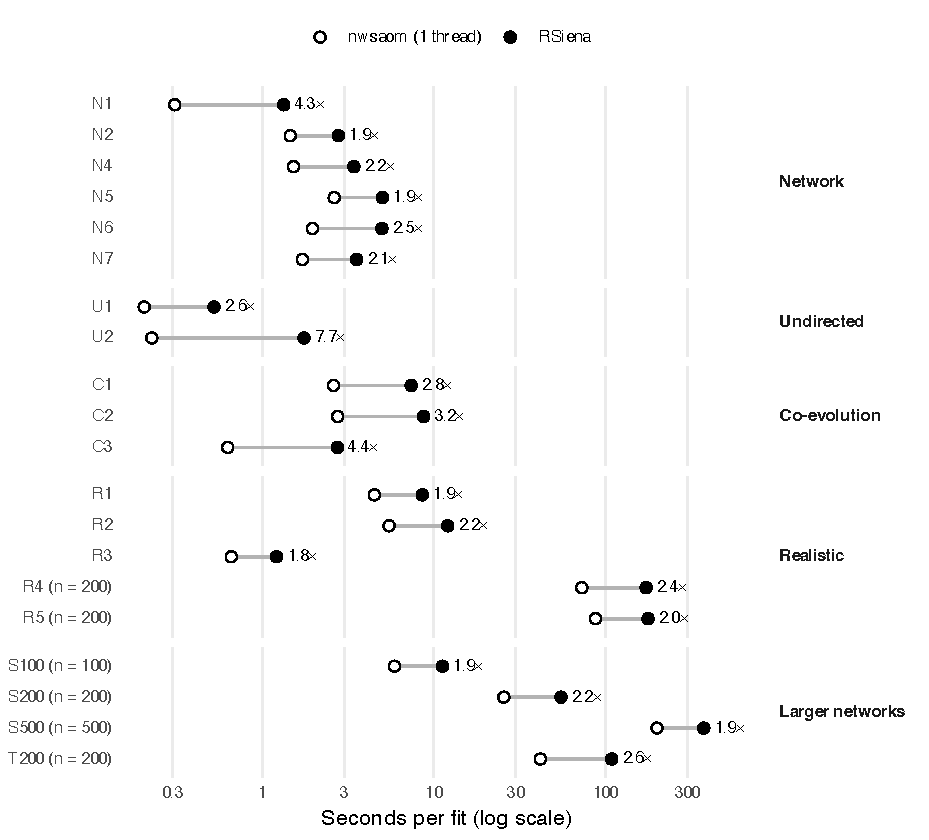
\includegraphics[width=\textwidth]{fig_bench_time.pdf}
\caption{Median seconds per fit (log scale): \nwsaom{} on one thread (open
circles), RSiena (filled circles).}
\end{figure}

\paragraph{Where the difference comes from.} RSiena runs the loop over about
2{,}200 network simulations per fit in R and calls its compiled code once per
simulation. Profiling shows that for N1 (\texttt{outdegree}, \texttt{reciprocity}) 36\% of its time
is compiled simulation and 64\% R overhead; for N2 (with \texttt{gwesp()}) 76\% and 24\%.
\nwsaom{} passes the data to its plugin once per fit and the plugin runs
whole batches of simulations, so the overhead nearly disappears. This explains
the largest gains for cheap-to-simulate models. For N2 removing the overhead
alone would give at most a factor 1.3; the observed \benchNtwoSp{} means the
simulation code itself is also faster.

\section{Further models}\label{sec:benchextra}

The same comparison, with the same conventions (default settings of both programs, one thread each, wall-clock seconds per fit, a fit counts as converged when RSiena's overall convergence ratio is below 0.25), for the later model families. The data are the Glasgow friendship panel, a second randomly generated network and the smoking behavior (several networks), and simulated bipartite data (two-mode). The table uses the median over three converged fits per program.

\begin{table}[htbp]
\centering
\caption{Further models: \texttt{nwsaom} and RSiena 1.6.6, both single-threaded, same data and effects:
largest difference in a mean estimate (in RSiena standard errors) and median seconds per fit over three converged fits}
\label{tab:benchextra}
\footnotesize
\begin{tabular}{l>{\raggedright\arraybackslash}p{0.34\textwidth}rrrrrr}
\toprule
 & Specification & $n$ & Waves & Max diff & \texttt{nwsaom} & RSiena & Speed-up \\
\midrule
\multicolumn{8}{l}{\textit{Two-mode}} \\
X1 & \texttt{outdegree}, \texttt{indegpopularity}, \texttt{cycle4} & 40$\times$20 & 3 & 0.06 & 1.00 & 2.82 & 2.8 \\
X2 & \texttt{outdegree}, \texttt{indegpopularity}, \texttt{outactivity}, \texttt{cycle4}, \texttt{outiso}, \texttt{antiiniso2} & 40$\times$30 & 3 & 0.04 & 0.45 & 0.63 & 1.4 \\
\addlinespace
\multicolumn{8}{l}{\textit{Two networks}} \\
X3 & both: \texttt{outdegree}, \texttt{reciprocity}; \texttt{crprod} & 50 & 3 & 0.07 & 1.62 & 3.93 & 2.4 \\
X4 & X3 without \texttt{crprod} + smoking: \texttt{linear}, \texttt{quadratic}, \texttt{avalt} (both networks) & 50 & 3 & 0.05 & 1.45 & 8.76 & 6.0 \\
X5 & X4 with \texttt{avalt} on network 1 only; \texttt{behegox}, \texttt{behaltx}, \texttt{behsim}, \texttt{samewwclosure:behavior} & 50 & 3 & 0.07 & 4.39 & 12.3 & 2.8 \\
X6 & undirected network 1 (\texttt{sym1}) + directed network 2; \texttt{crprod} & 50 & 3 & 0.07 & 1.20 & 3.26 & 2.7 \\
\addlinespace
\multicolumn{8}{l}{\textit{Single network}} \\
X7 & \texttt{outdegree}, \texttt{reciprocity}, \texttt{gwesp}, \texttt{samextranstrip()}, \texttt{altxoutact()}, \texttt{egoplusaltsqx()} & 50 & 3 & 0.04 & 3.06 & 4.33 & 1.4 \\
X8 & \texttt{outdegree}, \texttt{reciprocity}, \texttt{ownx(transtrip1 transrectrip2 jout)} & 50 & 3 & 0.07 & 1.73 & 2.85 & 1.6 \\
\bottomrule
\end{tabular}
\par\smallskip\footnotesize Medians over three converged fits (overall convergence ratio $<0.25$) per program; fits above the threshold were left out and replaced by the next seed (RSiena: X1 seed 3, X4 seeds 1--2, X5 seed 2; \texttt{nwsaom}: X8 seed 3). X1, X2: both programs unconditional (\texttt{unconditional}; \texttt{cond = FALSE}); X3--X6: \texttt{nwsaom multinet} with \texttt{k0(100) k3(1000)} against RSiena \texttt{n3 = 1000, nsub = 4}. Max diff includes the rate parameters.
\end{table}


All eight models agree with RSiena (the largest difference of a mean estimate, rates included, is 0.07 RSiena standard errors). The speed differs by family:
\begin{itemize}
\item \textbf{Several networks} (X3--X6) are 2.4 to 6.0 times as fast, most of all with a behavior and effects of the behavior on both networks (X4). A likely reason is the per-simulation overhead of RSiena's R code, which is paid for every dependent variable (see the profile at the end of the section on one thread); this was not profiled for these models.
\item \textbf{Newer single-network effects} (X7, X8) are 1.4 and 1.6 times as fast.
\item \textbf{Two-mode networks} are faster, but by less than the one-mode models: X1 takes 1.00 second in \nwsaom{} against 2.82 in RSiena, X2 0.45 against 0.63. Computing the four-cycle statistic for all alternatives of an actor at once made X1 2.5 times as fast as before (3.40 to 1.00 seconds, with the estimates unchanged to the last digit). Most of the time of X2 goes to the overhead around many short simulations, not to the simulation itself.
\end{itemize}
Some effect sets were chosen so that RSiena converges: on the 40$\times$20 data \texttt{outactivity} together with \texttt{indegpopularity} and \texttt{cycle4} does not converge in RSiena, \texttt{antiiniso2} on the same data and the effects \texttt{Jin} and \texttt{Jout} together on the Glasgow data make \texttt{siena07} stop with ``thetaBound should be set higher'', and the \texttt{Jout} estimate in X8 is large (about 9.6, standard error about 4) in both programs. Some fits did not converge in one of the programs (RSiena: X1 two of eight seeds, X4 and X5 two each, X8 one; \nwsaom{}: X8 one); they are left out of the table and replaced by the next seed. The machine was not completely idle while these timings were taken (load average 1.2 to 2.9), so small differences are noise.

\section{Why \nwsaom{} is faster}\label{sec:whyfast}
Both programs run the same algorithm: the same Robbins--Monro phases, the same number of simulations and the same ministep model. The speed-up comes from how the simulation is carried out.
\begin{itemize}
\item \textbf{The simulation loop runs in compiled code.} RSiena calls its compiled simulation once per simulated network from R, and the R code around it takes 24\% to 64\% of the time of the single-network models. \nwsaom{} hands the plugin whole batches of simulations, so this overhead largely disappears. This matters most for models that are cheap to simulate, which is why the largest single-network speed-ups are for \texttt{outdegree} and \texttt{reciprocity} models.
\item \textbf{The change statistics of an actor are computed together.} At each ministep an actor weighs all its possible tie changes. RSiena loops over the alternatives and, for each alternative, over the effects, and calls each effect's method on its own. The plugin turns the loops around: for each effect it passes once over all alternatives of the actor, in tight loops over arrays, and quantities that several alternatives share are computed once per actor instead of once per alternative (for example the number of two-paths through a tie, or the four-cycle count of the two-mode models). A tie lookup is an array access, because the plugin keeps each network as a dense adjacency matrix together with neighbor lists.
\item \textbf{Several networks share one simulation.} RSiena handles each dependent variable as a separate object with its own caches, and the cross-network effects reach into the other variable's cache. The plugin keeps all networks of a period in one structure and evaluates the cross-network terms on it directly. The models with several networks, the largest speed-ups of the tables, were not profiled in RSiena, so this is not claimed to be the whole explanation.
\end{itemize}
The explanations rest on the profile of RSiena's R and C++ time shares given above, on reading the RSiena source, and on the four-cycle experiment; RSiena's C++ code itself was not instrumented. The speed-up is smallest for the covariate models (1.4 to 1.6 times), where RSiena's per-effect code does little work per alternative and the difference is mostly the simulation loop.

\section{Using several cores}

RSiena can spread a fit over several R processes only on request
(\texttt{useCluster = TRUE, nbrNodes = $k$}); \nwsaom{} uses threads by default.

\begin{table}[htbp]
\centering
\caption{\texttt{nwsaom} with 1 to 10 threads: median seconds per fit over three seeds
(in parentheses, speed-up over one thread). Estimates are identical for every number of threads.}
\label{tab:cores}
\footnotesize
\begin{tabular}{lrrrrr}
\toprule
Model & $n$ & \texttt{cores(1)} & \texttt{cores(2)} & \texttt{cores(5)} & \texttt{cores(10)} \\
\midrule
R1 & 50 & 4.31 (1.0) & 3.44 (1.3) & 2.96 (1.5) & 2.86 (1.5) \\
R4 & 200 & 72.9 (1.0) & 56.5 (1.3) & 48.1 (1.5) & 45.2 (1.6) \\
R5 & 200 & 87.7 (1.0) & 49.7 (1.8) & 40.6 (2.2) & 38.7 (2.3) \\
\bottomrule
\end{tabular}
\end{table}


More threads help, less than proportionally: ten threads make R1 and R4 about
\coresRone{} and \coresRfour{} times as fast and the co-evolution model R5
\coresRfive{} times as fast. Phase~2 cannot be split across threads because each
Robbins--Monro step needs the previous estimate; only Phases~1 and~3 run fully in parallel.
Against single-threaded RSiena, \nwsaom{} with \texttt{cores(\coresmaxthreads)} is
\coresvsrsmin{} to \coresvsrsmax{} times as fast on these three models. The
estimates are identical for every number of threads, because each simulation's
random numbers depend only on the seed and the simulation's position.

\section{Limits of this benchmark}

\begin{itemize}
\item One machine and one data set (Glasgow and disconnected copies of it);
      speed-ups may differ for other effects and sparser or denser networks.
\item Both programs at default settings; RSiena's \texttt{nbrNodes} was only used
      where stated.
\item The further models of Section~\ref{sec:benchextra} are one specification per family; the timings of other effect sets and sizes may differ.
\item Older \texttt{nwsaom} versions simulated structural terms (e.g.\ transitive
      reciprocated triplets, outdegree assortativity) in Mata, which was up to
      two orders of magnitude slower than RSiena; with the native plugin these
      terms run at about RSiena's speed.
\end{itemize}
